\linespread{1.2}
\documentclass{beamer}
\usepackage{epstopdf}
\usepackage{tabularx}
\usepackage{amsmath}%
\usepackage{amscd} %allows drawing commutative diagrams
\usepackage{amsfonts}%
\usepackage{amssymb}%
\usepackage{graphicx}
\usepackage{color}

\newcommand{\noteLA}[1]{\textcolor{blue}{\footnotesize\textit{{noteLA: #1}}}} %this defines a new command for notes which has one argument
\def\noteLA #1{} %when activated, suppresses printing notes - remember to de-activate with %sign when sending draft text

\setbeamertemplate{navigation symbols}{}

%\usetheme{Rochester}
%\usetheme{Madrid}
%\usetheme{Goettingen}
%\usetheme{Singapore}
\usetheme{default}

\beamersetuncovermixins{\opaqueness<1>{25}}{\opaqueness<2->{15}}

\addtobeamertemplate{navigation symbols}{}{%
	\usebeamerfont{footline}%
	\usebeamercolor[fg]{footline}%
	\hspace{1em}%
	\insertframenumber/\inserttotalframenumber
}

\begin{document}
\title{Heterogeneity and the Distance Puzzle}  
\author[Archanskaia and Daudin]{Archanskaia E.\inst{*} and Daudin G.\inst{**}}
\institute{ \inst{*} KU Leuven
  \and
  \inst{**} PSL, LEDa, DIAL/SciencesPo, OFCE
}
\date{September 2019
%\today
\\
\vspace{.3cm}
%\textit{Congress of the European Economic Association, 2012}
} 
\begin{frame}[plain]
\titlepage
\end{frame}

%\section{Introduction} 
\begin{frame}[plain]\frametitle{Introduction: the paradox of distance}
\begin{itemize}
	\item The distance effect is increasing or stable through time in gravity models: Disdier  \&  Head, (2008), Head \& Mayer (2013)...
	\begin{itemize}
		\item This seems counter-intuitive ("Death of distance")
	\end{itemize}
	\item Various answers in the literature (see Head \& Mayer (2013)):
	\begin{itemize}
		\item Problem with the log-linear estimation strategy?
		\begin{itemize}
			\item Not taking zeros into account + heteroskedasticity 
			\item $\Rightarrow$ PPML estimates (Santo Silva \& Tenreyro (2006), , Bosquet \& Boulhol (2015))
		\end{itemize}
		\item Composition effect (Larch et al. (2016))
		\item Relative evolution of short-distance trade costs compared to long-distance trade costs (Buch \& al. (2004), Krautheim (2012))
		\item Input-output linkage (Daudin et al. (2011))
		\item Network : the distance coefficient does not depend on trade costs (Chaney (2018))
	\end{itemize}
\end{itemize}
\end{frame}

\begin{frame}[plain]\frametitle{How do we contribute?}
	\noteLA{Say here: world may be getting smaller while at the same time the elasticity of trade to distance may be non-decreasing. This is where ambiguity in distance puzzle appears.}
\begin{itemize}
	\item Every theoretical fundation of the gravity equation delivers a relationship between the distance elasticity and a degree of structural heterogeneity in some model-specific structural dimension
		\begin{itemize}
			\item "Trade elasticity" (Arkolakis et al. (2012))
		\end{itemize}
	\item The distance coefficient is the product of:
	\begin{enumerate}
		\item The elasticity of distance to trade costs
		\item The elasticity of trade to trade costs
	\end{enumerate}
	\item Empirical evidence on the historical evolution of structural heterogeneity is notoriously scarce
		\begin{itemize}
			\item The only other try we know of is Berthelon \& Freund (2008) from the late 1980s to early 2000s
		\end{itemize}
	\item We document over 1962-2013 how the increasing substituability of the bundles shipped out by each country contributes to the paradox in the Armington framework
\end{itemize}
\end{frame}



\begin{frame}[plain]\frametitle{Dispersion of the number of products exported by each country}
\begin{figure}
	\begin{center}
		\setlength{\fboxrule}{1pt} %makes border lines thick
		\setlength{\fboxsep}{.1in} %increases distance to border
		\fbox{\includegraphics[trim = 0mm 0mm 0mm 0mm, clip, height=2.5in]{vioplot.pdf}}
	\end{center}
\end{figure}
\end{frame}



\begin{frame}[plain]\frametitle{Standard deviation in the number of products exported by each country }
\begin{figure}[h!]
	\begin{center}
		\setlength{\fboxrule}{1pt} %makes border lines thick
		\setlength{\fboxsep}{.1in} %increases distance to border
		\fbox{\includegraphics[trim = 0mm 0mm 0mm 0mm, clip, height=2.5in]{Fall_of_SD.pdf}}
	\end{center}
\end{figure}
\end{frame}

\begin{frame}
	\frametitle{Overview} 
	\tableofcontents
\end{frame}


\begin{frame}[plain]\frametitle{Summary of results}
\vspace{0.3cm}
\begin{itemize}
\item Robustness of distance puzzle in 1962-2013: increase in distance coefficient between +5\% and +31\%
%Working with COMTRADE bilateral trade data at the 4-digit level 
\vspace{0.3cm}
\item Evolution of heterogeneity parameter:increase between +22\% and +81\%
\vspace{0.3cm}
\item Elasticity of trade costs to distance has not increased
\vspace{0.3cm}
\item Which dimension of increased country similarity? 
	\begin{itemize}
	\item Result obtained within the Armington framework 
	\item Increased substitutability of country-specific product bundles 
	\end{itemize}
%Reduced heterogeneity means increased substitutability of exporter-specific product bundles
\end{itemize}

\end{frame}
%motivation of presenting results for 1970-2009: period in which air transportation has become an important transport means in trade
%message in one sentence: evolution of heterogeneity parameter provides direct explanation of increase distance elasticity of trade while composition and sample effects deepen the distance puzzle (composition: consistent with increasing share of manuf goods in trade (commodities and reference priced goods are more substitutable); sample: consistent with idea that countries which are stable trade partners may have witnessed relatively more similarity of export bundles than if all changes in sample of trading pairs allowed). Notice that cumulated effect composition and sample still at +14\% which means that stable partners are maybe also those which have experienced less changes in terms of composition of traded goods (manuf already in 62, and therefore no additional kick from composition effects). Thus, our analysis of composition and sample effects does tell a convincing story about world trade patterns: for unstable partners, more heterogeneity in bundles but stronger increase in share of manuf overtime; for stable partners, less movement in share of manuf but more movement in terms of reduced heterogeneity of exchanged varieties in manuf. 
%Not useful to say but say if questioned: For this parameter to be true trade elasticity across models would correspond to a very strong assumption on fixed trade costs: so small that all firms enter all export markets, and therefore only intensive margin matters.
%think about Egger argument about home bias: mechanical increase in distance sensitivity of trade flows as countries grow?

\begin{frame}[plain]\frametitle{Roadmap}\tableofcontents
\end{frame} 
%Say: I will go quickly over documenting the presence of distance puzzle in our data b/c this finding is present in several papers. The objective is to have sufficient time to explain our estimation methodology and results on the evolution of the heterogeneity parameter.

\section{The distance puzzle in our data}
\subsection{Benchmark estimation}
\begin{frame}\frametitle{Estimation procedure (1)}
\begin{itemize}
	\item We run gravity equations (obviously)
	\begin{itemize}
		\item COMTRADE data, 1962-2009 STIC 4 digits (1962-2009 )
		\item cross section, no panel
		\item focus on evolution of distance elasticity overtime
		\item using the PPML estimator (for consistency \& efficiency)
	\end{itemize}
\item Microfounded gravity equation (Anderson \& Wincoop (2003)):
\begin{eqnarray}
X_{ij,t} & = & \left(\frac{Y_{i,t}Y_{j,t}}{Y_t}\right)\left(\frac{\tau_{ij,t}}{\Pi_{i,t}P_{j,t}}\right)^{\epsilon_t} \nonumber
\end{eqnarray}
%where the above formula is the standard gravity equation which can be derived across frameworks
\item heterogeneity parameter: $\epsilon_t$: $1-\sigma_{t}$ in Armington (sector or firm productivity heterogeneity in the frameworks respectively of Eaton \& Kortum and Melitz/Chaney)
%$X_{ij,t}$ is the value of goods from country $i$ consumed in country $j$ in year $t$, i.e. bilateral imports at cif prices. Imports are a function of the nominal income of each trading partner $Y_{ij,t}$ and $Y_{j,t}$, of world income $Y_t$, of bilateral trade costs $\tau_{ij,t}$, and of inward and outward multilateral trade resistance terms $\Pi_{i,t}$, $P_{j,t}$. 
\end{itemize}
\end{frame}

\begin{frame}[plain]\frametitle{Estimation procedure (2)}
\begin{itemize}
\item Trade costs: 
	\begin{itemize}
	\item distance parameter: $\eth_{ij}$
	\item time-invariant cost vector of controls (adjacency,...): $Z_{ij}$
	\item time-varying cost vector of controls (same country, colonial status,...): $S_{ijt}$
	\item unobserved bilateral trade cost component assumed to have mean zero conditional on the observables: $\nu_{ijt}$ 
	%potentially time-varying, therefore includes same country, colonial linkages, so on
\begin{gather}
\tau_{ijt}=\exp\left\{\rho_t\ln{\eth_{ij}}+{Z_{ij}}\zeta_{t}+{S_{ijt}}\varsigma_{t}+\nu_{ijt}\right\} \nonumber
\end{gather}
	\item $\rho_t$ is the `world shrinkage' parameter \\ 
\hspace{1cm} i.e. elasticity of trade costs to distance
	\end{itemize}
% (`shrinkage') 
%As is standard in the gravity literature, we model bilateral trade costs as a function of bilateral distance $dist_{ij}$, a vector $Z_1$ of bilateral trade cost controls such as adjacency, common language, colonial linkages, belonging or having once belonged to the same country, and a vector $Z_2$ of trade cost controls linked to trade policy such as common membership of GATT/WTO and common membership of an FTA.
\item Estimated equation:
\begin{gather}
X_{ij,t}=\exp{\left(\xi_t-\delta_{t}\ln{\eth_{ij}}+{Z_{ij}}\tilde{\zeta_{t}}+{S_{ijt}}\tilde{\varsigma_{t}}+f_{it}+f_{jt}\right)\eta_{ijt}} \nonumber
\end{gather}
%multiplicative model
	\begin{itemize}
	\item $f_{it}$ and $f_{jt}$are fixed effects to control for price levels
	\item $\xi_{ijt}$ is a multiplicative error term which includes the exponentiated unobserved bilateral trade cost
	\item distance elasticity: $-\delta_{t}=\epsilon_{t}\rho_t$
%exporter and importer dummies: $fe_{i,t}$, $fe_{j,t}$
%\item Baseline: trade policy controls excluded (FTAs)
	\end{itemize}
\end{itemize}
\end{frame}

\begin{frame}[plain]\frametitle{Baseline regression (PPML)}
\begin{figure}[h!]
%\caption{Distance coefficient in the baseline PPML regression \label{fig:distcoefbaseline}}
\begin{center}
\setlength{\fboxrule}{1pt} %makes border lines thick
\setlength{\fboxsep}{.1in} %increases distance to border
\fbox{\includegraphics[trim = 0mm 0mm 0mm 9.5mm, clip, height=2.5in]{DP_baseline.pdf}}
\end{center}
\end{figure}
%\vspace{0.3cm}
%8\% increase in distance elasticity
Increase in absolute value of 4.5\%
\end{frame}

\subsection{Composition and sample effects}
\begin{frame}\frametitle{Sample composition effect}
\begin{itemize}
\item We know the country sample potentially matters
	\begin{itemize}
	\item Increasing number of new low volume long-distance relationship
	\item Potentially increases the distance elasticity of trade (Mayer et al. (2019), Head \& Mayer (2013) ) 
	\item Though it should be less of an issue with PPML
	\end{itemize}
\item There are big sample issues in the data	
\item Test: keep only trading pairs that have reciprocal non-zero trade every year from 1962 to 2009 ("Superbalanced sample")
%similar results if square: all with all in each year
	\begin{itemize}
	\item It deepens the puzzle 
	\end{itemize}
\end{itemize}
\end{frame}



%interpretation of composition and sample effects.
%composition: consistent with increasing share of manuf goods in trade (commodities and reference priced goods are more substitutable); sample: consistent with idea that countries which are stable trade partners may have witnessed relatively more similarity of export bundles than if all changes in sample of trading pairs allowed). Notice that cumulated effect composition and sample still at +14\% which means that stable partners are maybe also those which have experienced less changes in terms of composition of traded goods (manuf already in 62, and therefore no additional kick from composition effects). Thus, our analysis of composition and sample effects does tell a convincing story about world trade patterns: for unstable partners, more heterogeneity in bundles but stronger increase in share of manuf overtime; for stable partners, less movement in share of manuf but more movement in terms of reduced heterogeneity of exchanged varieties in manuf. 
\begin{frame}[plain]\frametitle{Share of active pairs}
\begin{figure}[h!]
\begin{center}
\setlength{\fboxrule}{1pt} %makes border lines thick
\setlength{\fboxsep}{.1in} %increases distance to border
\fbox{\includegraphics[trim = 0mm 0mm 0mm 9.5mm, clip,height=2.5in]{part1_active_pairs.eps}}
\end{center}
\end{figure}
\end{frame}


\begin{frame}[plain]\frametitle{Superbalanced sample}
	\begin{figure}[h!]
		\begin{center}
			\setlength{\fboxrule}{1pt} %makes border lines thick
			\setlength{\fboxsep}{.1in} %increases distance to border
			\fbox{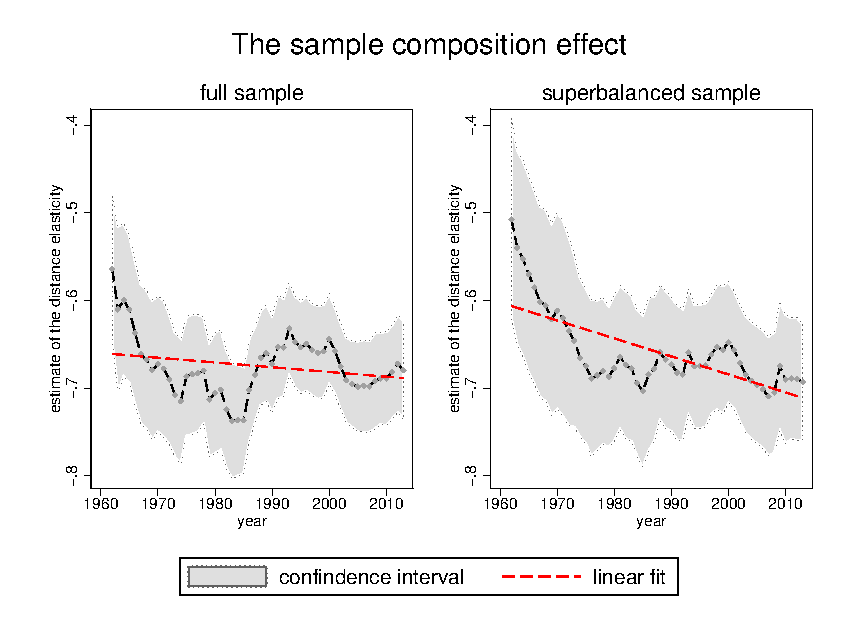
\includegraphics[trim = 0mm 0mm 0mm 9.5mm, clip,height=2.5in]{sample_composition_effect_1962.eps}}
		\end{center}
	\end{figure}
Increase in absolute value of 18.2\%
\end{frame}





\begin{frame}[plain]\frametitle{Sector composition}

\begin{itemize}
	\item We do not expect the elasticity of trade to distance to be constant by sector
	\begin{itemize}
		\item Some sectors can only be procured in specific places (oil), other are more mobile (textile)
		\item In the long-term, the decline of the share of oil should increase the absolute value of the elasticity of trade to distance
		\item In the short-term, price variation of primary products change their share in trade and hence the elasticity of trade to distance
	\end{itemize}
	\item We use two tests
	\begin{enumerate}
		\item Fixing the sectoral compositon of total trade to 1962. We modify all trade flows by a sector-specific factor.
		\begin{eqnarray}
		\tilde{X}^k_{ijt}=X^k_{ijt}*\frac{s^k_{w,1962}}{s^k_{w,t}} \nonumber
		\end{eqnarray}
		\item Fixing the sectoral composition of each country's export to 1962. We modify all trade flows by a sector and country-specific factor
		\begin{eqnarray}
		\tilde{X}^k_{ijt}=X^k_{ijt}*\frac{s^k_{i,1962}}{s^k_{i,t}} \nonumber
		\end{eqnarray}
	\end{enumerate}
\end{itemize}

\end{frame}

\begin{frame}[plain]\frametitle{Product composition effect: fixing the world bundle}
	\begin{figure}[h!]
		\begin{center}
			\setlength{\fboxrule}{1pt} %makes border lines thick
			\setlength{\fboxsep}{.1in} %increases distance to border
			\fbox{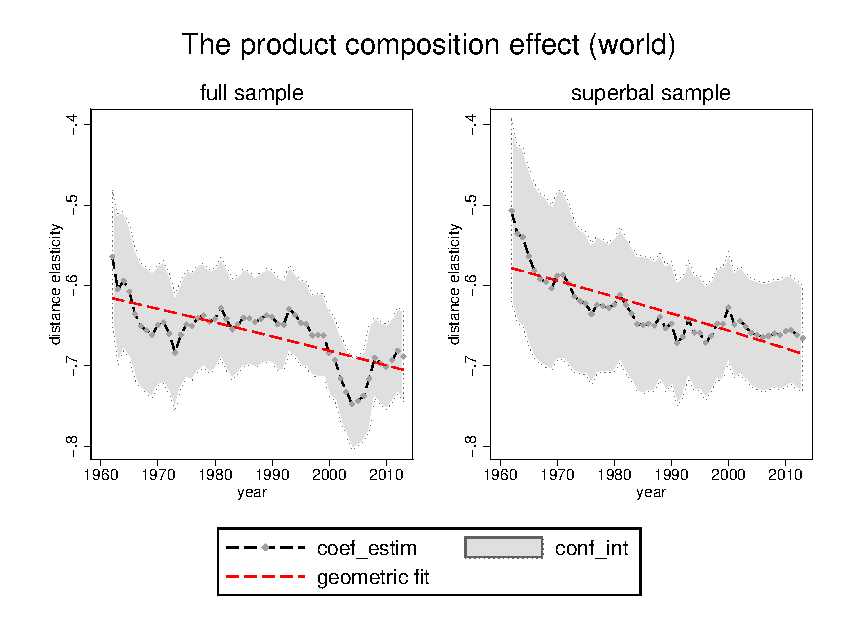
\includegraphics[trim = 0mm 0mm 0mm 9.5mm, clip,height=2.5in]{product_composition_effect_world_1962.eps}}
		\end{center}
	\end{figure}
	Increase in absolute value of 14.5 and 18.4\%
\end{frame}

\begin{frame}[plain]\frametitle{Product composition effect: fixing the country  bundle}
	\begin{figure}[h!]
		\begin{center}
			\setlength{\fboxrule}{1pt} %makes border lines thick
			\setlength{\fboxsep}{.1in} %increases distance to border
			\fbox{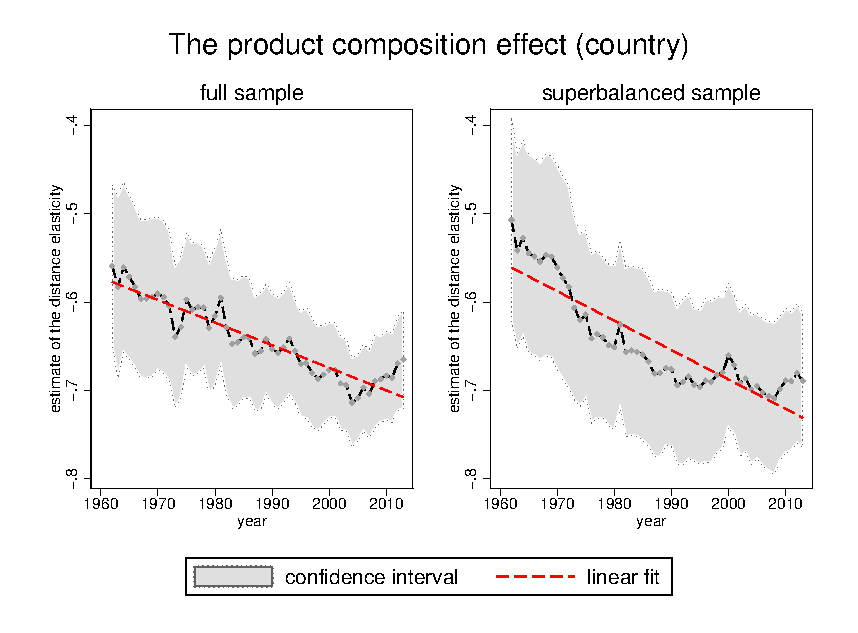
\includegraphics[trim = 0mm 0mm 0mm 9.5mm, clip,height=2.5in]{product_composition_effect_country_1962.eps}}
		\end{center}
	\end{figure}
	Increase in absolute value of 22.7 and 31.4\%
\end{frame}






\begin{frame}[plain]\frametitle{Summary (PPML)}
\begin{table}[H]
	\caption{Evolution of $\delta_t$: sample and composition effecs \label{tab:part1recap}}
	\scriptsize
	\begin{center}
		\begin{tabular}{|l|c|c|c||c|c|c|}
			\hline
			& \multicolumn{3}{|c||} {FULL} & \multicolumn{3}{|c|} {STABLE} \\
			\hline
			& {rate (\%)} & {R-sq} & {total change} & {rate (\%)} & {R-sq} & {total change} \\
			\hline
			Baseline  & $.09^{*}$ & $.07$ & $1.045$ & $.33^{***}$ & $.49$     & $1.182$ \\
			\hline
			World bundle & $.26^{***}$ & $.53$ & $1.145$ & $.33^{***}$ & $.68$ & $1.184$ \\
			\hline
			Country bundle & $.40^{***}$ & $.87$ & $1.227$ & $.54^{***}$ & $.77$ &  $1.314$ \\
			\hline
			\multicolumn{7}{|l|}{\begin{tiny} Note: Estimated annualized growth rates reported in col.2 and col.5 are obtained as a geometric fit on the\end{tiny}} \\
			\multicolumn{7}{|l|}{\begin{tiny} basis of annual point estimates of the distance coefficient in 1962-2013.
					Col.3 and col.6 report the share \end{tiny}} \\
			\multicolumn{7}{|l|}{\begin{tiny} of time variation in the point estimate explained with the annualized growth rate.
			\end{tiny}} \\
			\hline
		\end{tabular}  
	\end{center}
\end{table}
\end{frame}
%share of total trade within FTAs increases from less than 20\% to more than 40\% of trade between 1962-2009 while the share of trade between countries situated closeby (less than 2000 km: first decile of distance distribution of trade) which takes place within FTAs has increased from 38 to 79\% over the same period.
\if 0
\begin{frame}[plain]\frametitle{Robustness of puzzle}
\vspace{0.3cm}
\begin{itemize}
\item Combining the three effects:
\item dominated by FTA: makes puzzle disappear
\item but explanation unsatisfactory (endogeneity; proximity controls)
\vspace{.3cm}
\item Admit growing role of distance is robust
\item what does this mean?
\end{itemize}
\end{frame}
\fi

\section{Interpreting the distance coefficient}
\subsection{What does the trade elasticity actually measures?}
\begin{frame}\frametitle{Ingredients of the puzzle}
\begin{itemize}
\vspace{0.3cm}
\item The distance coefficient is the elasticity of trade to distance
\begin{itemize}
\item Trivial: the whole point of log-linear equations
\item Still the case in the PPML specification
\end{itemize}
\vspace{0.3cm}
\item It is a product of two coefficients:
\begin{itemize}
\item Elasticity of trade flows to trade costs $\epsilon$
\item Elasticity of trade costs to distance $\rho$
\end{itemize}
\vspace{0.3cm}
\item The `death of distance' intuition is really about the elasticity of trade costs to distance (Which should be going down)
\item But it does not tell much about the heterogeneity dimension, i.e. the trade elasticity $\epsilon$
\end{itemize}
\end{frame}

\begin{frame}[plain]\frametitle{Short incursion in microfoundations (1)}
\begin{itemize}
\item The gravity equation can be justified by three canonical families of theories: (see Head \& Meyer(2014) )
\item Ricardian framework (Eaton \& Kortum (2002))
	\begin{itemize}
	\item Homogeneous goods
	\item Shop around the world for lowest cost supplier (intersectoral productivity heterogeneity)
	\end{itemize}
\item Heterogeneous firms framework: (Melitz (2003),  Chaney (2008))
	\begin{itemize}
	\item Trade because all firms produce different varieties
	\item A subset of firms enters export markets (intrasectoral productivity heterogeneity)
	\end{itemize}
\item Armington framework (Anderson and Wincoop (2003))
	\begin{itemize}
	\item Trade because consumers value variety 
	\item Country-specific goods (heterogeneity: degree of substitutability between bundles)
	\end{itemize}
%\vspace{0.3cm}
%\item Consequences for the elasticity of trade to trade costs?
\end{itemize}
\end{frame}
%All theoretical frameworks used to derive the gravity equation are characterized by a common feature: the elasticity of trade flows to trade costs, the `trade elasticity', is decreasing in the degree of heterogeneity observed in a single dimension, and it is this dimension which is framework-specific. In the Ricardian framework, heterogeneity is intra-country and inter-sector: it measures the degree of dispersion in production efficiency within countries across goods, with the dispersion parameter assumed common across countries and sectors. In the Armington framework, the dimension of heterogeneity is the flipside of the Ricardian framework. Heterogeneity is inter-country and intra-sector, and corresponds to the parameter which measures the degree of perceived substitutability of country-specific varieties of each good. In the monopolistic competition framework with firm heterogeneity, the dimension of heterogeneity is intra-country and intra-sector. It is captured by the parameter which measures the degree of dispersion in firm productivity within a given sector, and this parameter is assumed common to all countries.
\begin{frame}[plain]\frametitle{Short incursion in microfoundations (2)}
\begin{itemize}
\item Ricardian framework: 
	\begin{itemize}
	\item Distance coefficient: $\rho\theta$
	\item $\theta$ captures intersectoral productivity dispersion
	\item if sectors have similar productivity \\ $\rightarrow$ small differences in variable costs have a large effect on trade flows
	\\ $\rightarrow$ high elasticity of trade to trade costs
	\end{itemize}
\item Monopolistic competition between heterogeneous firms:
	\begin{itemize}
	%\item assume fixed costs of trade are not distance-dependent
	\item Distance coefficient: $\rho\gamma$
	\item $\gamma$ captures productivity dispersion across firms (parameter of Pareto)
	\item if distribution decays swiftly, higher probability that productivity cut-off for exporting is close to the mass of firms \\ $\rightarrow$  small differences in variable costs have large effect on entry 
	\\ $\rightarrow$ high elasticity of trade to trade costs
	\end{itemize}
\end{itemize}
\end{frame}

\begin{frame}[plain]\frametitle{Short incursion in microfoundations (3)}
\begin{itemize}
\item Armington framework
	\begin{itemize}
	\item Distance coefficent:  $\rho(1-\sigma)$
	\item $\sigma$ captures degree of similarity between country-specific product bundles
	\item if the set of goods produced by different countries is similar \\ $\rightarrow$ high Armington elasticity 
	\\ $\rightarrow$ high elasticity of trade to trade costs
	\end{itemize}
\item In all cases: elasticity of trade flows to trade costs is inversely related to heterogeneity 
\end{itemize}
\end{frame}

\subsection{What do we know about the evolution of the trade elasticity?}

\begin{frame}\frametitle{Measuring the trade elasticity (1)}

\begin{itemize}
\item Evolution on the supply side
	\begin{itemize}
	\item Technological dissimilarity in productivity between sectors or firms
	\item Levchenko \& Zhang (2016) 1960-2010 in 75 countries: within-country convergence in knowledge shocks between sectors (but not the Eaton \& Kortum parameter)
	\item Andrews et al. (2016) 1997-2014 OECD: divergence between firm productivity inside sectors. But there are difficulties in interpreting it in the Meltiz framework
	\end{itemize}
\item Evolution on the demand side
	\begin{itemize}
	\item Welsch (2006): among exporters to the French market the lower-tier Armington elastiticy peaked in the 1970s and declined thereafter
	\item Broda et al. (2006): compares American imports between 1972-1988 and 1990-2001 they find a decrease
	\item These results would deepen the distance puzzle
	\end{itemize}
\end{itemize}
\end{frame}	

\begin{frame}\frametitle{Measuring the trade elasticity (2)}	
	\begin{itemize}
		\item Measuring the level of Armington elasticity
		\begin{itemize}
			\item A perenial question in trade economics from Feenstra (1994) to the review in Feenstra (2018)
			\item The canonical method assumes that it is constant through time: that is not interesting for us
			\item Feenstra's elasticity parametre determines short-run, marginal, longitudinal effects, whereas we are interested in the parameter that determines long-run, equilibrium, cross-section outcomes
		\end{itemize}
		\item Our method
		\begin{itemize}
			\item Measure the evolution of Armington elasticites
			\begin{itemize}
				\item (Its irrelevance in the Meltiz and Eaton \& Kortum framework is linked to the specific distribution functon of productivity)
			\end{itemize}
			\item uses cif unit values and bilateral trade flows to estimate the trade elasticity
			\item we need a measure of the aggregate level: that cannot be generally mimicked by a theoretically grounded weighted average of sector-specifie trade elasticities. So we assume they are all the same and work on agregrate data (Imbs \& Mejean (2015)).
		\end{itemize}
	\end{itemize}
\end{frame}	


%
%
%\item Features of our data: information on bilateral trade flows and unit values
%\item To measure efficiency heterogeneity: need information on domestic prices 
%\begin{itemize}
%\item intuition: country-specific cut-off for entry common to all exporters 
%\item price distribution in destination across all sources needed to estimate shape parameter of productivity distribution
%\end{itemize}
%\vspace{0.3cm}
%\item However we can measure substitutability across frameworks
%\begin{itemize}
%\item use variation of market shares of country-level composite goods across export markets 
%\item construct relative prices of product bundles
%\item estimate the aggregate Armington elasticity in cross section
%\end{itemize}
%\item The estimated parameter is the trade elasticity in the Armington framework
%\end{itemize}
%\end{frame}
%\noteLA{Say: for this parameter to be valid across frameworks means making a strong assumption on fixed costs of trade: so small that all export}
%%\subsection{Consistent aggregation procedure to get relative prices}
%\noteLA{Say: in Armington model, producer heterogeneity not modelled: source-specific cost component gives directly the price of the exported good: trade elasticity can be estimated using source-specific price distributions}

\begin{frame}[plain]\frametitle{Our equation (1)}
\begin{itemize}
%	\item One-good Armington framework. ${X}_{ij}$ is the cif value of the exports from $i$ to $j$:
%	\[{{X}_{ij}}={{\left( \frac{{{P}_{ij}}}{{{P}_{j}}} \right)}^{1-\sigma}}{{Y}_{j}}\]
%	${{P}_{ij}}$ is the cif price and ${{P}_{j}}$ is the price index in the destination and ${{Y}_{j}}$ total import demand in the destination.
%	The exponent $\left( 1-\sigma \right)$ is the trade elasticity
	\item Aggregate exports are the sum of imports from each sector $k$ where a sector corresponds to a SITC 4-digit category: ${{X}_{ij}}=\sum\limits_{k}{{{X}_{k,ij}}}$.
	Sectoral demand in country  in sector  for imported goods is given by: 
	\[\begin{array}{*{35}{l}}
	{{Y}_{k,j}} & = & {{\left( \frac{{{P}_{k,j}}}{{{\beta }_{k}}{{P}_{j}}} \right)}^{1-\sigma }}{{Y}_{j}}  \\
	\end{array}\]
	Where ${{P}_{k,j}}$ and ${{P}_{j}}$ are price indexes, ${{\beta }_{k}}>0$ is a sector-specific preference parameter, ${{Y}_{j}}$ is total demand for imported goods, $\sigma >1$ is the elasticity of substitution between sectors, and the exponent $\left( 1-\sigma \right)$ is the trade elasticity
	\item Each country exports a specific national variety. Preferences within each sector $k$ between national varieties are assumed well represented by a CES utility function with the same $\sigma $ parameter as the intersectoral CES utility function.
\end{itemize}
\end{frame}



\begin{frame}[plain]\frametitle{Our equation (2)}
\begin{itemize}
\item Intrasectoral demand for varieties exported by $i$ in $j$ in sector $k$ is: 
\[\begin{array}{*{35}{l}}
{{X}_{k,ij}} & = & {{\left( \frac{{{p}_{k,ij}}}{{{\gamma }_{i}}{{P}_{k,j}}} \right)}^{1-\sigma }}{{Y}_{k,j}}  \\
\end{array}\]
Where ${{\gamma }_{i}}>0$ is a origin-country-specific preference parameter and ${{P}_{k,j}}$ is the CES price index:
\[\begin{array}{*{35}{l}}
{{P}_{k,j}} & = & {{\left[ \sum\limits_{i\ne j}{{{\left( \frac{{{p}_{k,ij}}}{{{\gamma }_{i}}} \right)}^{1-\sigma }}} \right]}^{1/(1-\sigma )}}  \\
\end{array}\]
\item Defining $\frac{{{Y}_{k,j}}}{{{Y}_{j}}}={{\omega }_{k,j}}$, we get: 
\[\begin{array}{*{35}{l}}
\frac{{{X}_{k,ij}}}{{{Y}_{j}}} & = & {{\omega }_{k,j}}{{\left( \frac{{{p}_{k,ij}}}{{{\gamma }_{i}}{{P}_{k,j}}} \right)}^{1-\sigma }}  \\
\end{array}\]
\item Summing over all SITC 4-digit sectors: 
\[\begin{array}{*{35}{l}}
\sum\limits_{k=1}^{K}{\frac{{{X}_{k,ij}}}{{{Y}_{j}}}}=\frac{{{X}_{ij}}}{{{Y}_{j}}} & = & \gamma _{i}^{\sigma -1}\sum\limits_{k=1}^{K}{{{\omega }_{k,j}}}{{\left[ \frac{{{p}_{k,ij}}}{{{P}_{k,j}}} \right]}^{1-\sigma }}  \\
\end{array}\]
\end{itemize}
\end{frame}



\begin{frame}[plain]\frametitle{Our equation (3)}

\begin{itemize}
\item Changing notation to $\kappa_i=\gamma_i^{\sigma-1}$, the market share becomes, assuming multiplicative errors of measurement:

%\begin{eqnarray}
%\frac{{X}_{ij}}{Y_j} & = & {{\kappa }_{i}}\sum\limits_{k=1}^{K}{{{\omega %}_{k,j}}}\frac{p_{k,ij}^{1-\sigma }}{\sum\limits_{l\ne j}{{{\kappa }_{l}}}p_{k,lj}^{1-\sigma %}}  
%\end{eqnarray}

%As this is a market share, it is reasonable to assume that the errors are multiplicative.
%Measurement errors on a market share of 1\% cannot be the same in percentage points as measurement errors on a market share of 10\%.
%We have to fit the following model to the data:
\begin{eqnarray}
\frac{{{X}_{ij}}}{{{Y}_{j}}} & = & {{\kappa }_{i}}\sum\limits_{k=1}^{K}{{{\omega }_{k,j}}}\frac{p_{k,ij}^{1-\sigma }}{\sum\limits_{l\ne j}{{{\kappa }_{l}}}p_{k,lj}^{1-\sigma }}.{{e}^{{{\varepsilon }_{i,j}}}} \nonumber
\end{eqnarray}

%Notice that we only have non-zero observations, as ${{p}_{k,ij}}$ is only observed when there is a trade flow.
\item We take logs to transform the errors into additive ones and estimate the following equation with a non-linear least square procedure year by year:
\begin{eqnarray}
\ln \left( \frac{{{X}_{ij}}}{{{Y}_{j}}} \right) & = & \ln {{\kappa }_{i}} +\ln \left( \sum\limits_{k=1}^{K}{\frac{{{Y}_{k,j}}}{{{Y}_{j}}}.}\frac{p_{k,ij}^{1-\sigma }}{\sum\limits_{l\ne j}{{{\kappa }_{l}}}p_{k,lj}^{1-\sigma }} \right) +{{\varepsilon }_{i,j}}
\end{eqnarray}

\item This approach yields annual estimates of ${{\kappa }_{i}}$ and $\sigma $.
\end{itemize}
\end{frame}



%\begin{frame}[plain]\frametitle{Relative prices of product bundles}
%\begin{itemize}
%\item Consistent aggregation procedure to get relative prices
%\begin{itemize}
%\item CES preferences at inter- and intrasectoral level
%\item Intra- and intersectoral elasticities assumed equal
%\item Write sector-specific demand equation 
%\item Sum across all sectors 
%%\item Use approximation that for large number of sectors, log of sum approx. equal to sum of logs
%%(Imbs and Mejean)
%\end{itemize}
%\item Gives market share equation for aggregate bilateral trade as a function of the weighted average of sectoral relative prices of exporter in destination
%\begin{eqnarray}
%\ln\left[\frac{X_{ij}}{Y_j}\right]&\approx&-(\sigma-1)\ln\left[\sum_{k=1}^K{\omega_{j}(k)\frac{P_{ij}(k)}{P_j(k)}}\right] \nonumber
%\end{eqnarray} 
%\item Exponentiating gives equation estimated in Poisson:
%\begin{eqnarray}
%X_{ij}/Y_{j}&=&\exp{\left[\lambda_{0}-(\sigma-1)\ln{\left(\sum_{k}\omega_k\frac{P_{ij}(k)}{P_{j}(k)}\right)}+fe_{i}+fe_{j}\right]}\eta_{ij} \nonumber
%\end{eqnarray}
%\end{itemize}
%\end{frame}

\section{Evolution of the Armington trade elasticity}
\subsection{Benchmark and robustness estimation}

\begin{frame}[plain]\frametitle{Results}
\begin{itemize}
	\item Benchmark results: $|1-\sigma|$ has increased by 22\% from 1962 to 2013
	\begin{itemize}
		\item Point estimate in the low range $|1-\sigma|\in\left\{.4,.5\right\}$
		\item For the US, Feenstra (2018) obtain a point estimate in the $\left\{0.5,3\right\}$ range, depending on the estimator used,
		\item Imbs \& Mejean (2015) obtain a point estimate of $1-\sigma=-2$
	\end{itemize}
	\item Missing unit values: Trade flow observed, but no information on unit prices 
	\begin{itemize}
		\item we use a stepwise precedure to evaluate missing unit values from similar products
		\item $|1-\sigma|$ has increased by 35\% from 1962 to 2013
	\end{itemize}
	\item Zero trade flows: from 96.5\% to 91\%
	\begin{itemize}
		\item A priori not compatible with the Armington framework: we assume a statistical collection threshold
		\item To test the robustness of our result, we use the superbalanced sample: the share of zero trade flows is much smaller (but the rate of decline is similar)
		\item $|1-\sigma|$ has increased by 69\% from 1962 to 2013
	\end{itemize}
	\item Bad data ? The increase is faster in BACI (1995-2016): +1.18\% a year instead of +.4\%
\end{itemize}
\end{frame}


\begin{frame}[plain]\frametitle{Benchmark results}
	\begin{figure}[h!]
		\begin{center}
			\setlength{\fboxrule}{1pt} %makes border lines thick
			\setlength{\fboxsep}{.1in} %increases distance to border
			\fbox{\includegraphics[trim = 0mm 0mm 0mm 9.5mm, clip,height=2.5in]{"1ere regression 3e partie_baseline".pdf}}
		\end{center}
	\end{figure}
\end{frame}

\begin{frame}[plain]\frametitle{Trade with missing unit values}
	\begin{figure}[h!]
		\begin{center}
			\setlength{\fboxrule}{1pt} %makes border lines thick
			\setlength{\fboxsep}{.1in} %increases distance to border
			\fbox{\includegraphics[clip,height=2.5in]{Graph_missing_uv.pdf}}
		\end{center}
	\end{figure}
\end{frame}


\begin{frame}[plain]\frametitle{Imputed unit values}
	\begin{figure}[h!]
		\begin{center}
			\setlength{\fboxrule}{1pt} %makes border lines thick
			\setlength{\fboxsep}{.1in} %increases distance to border
			\fbox{\includegraphics[clip,height=2.5in]{"1ere regression 3e partie_prix_calc".pdf}}
		\end{center}
	\end{figure}
\end{frame}

\begin{frame}[plain]\frametitle{The prevalence of zero trade flows}
	\begin{figure}[h!]
		\begin{center}
			\setlength{\fboxrule}{1pt} %makes border lines thick
			\setlength{\fboxsep}{.1in} %increases distance to border
			\fbox{\includegraphics[clip,height=2.5in]{"graph_ztf".pdf}}
		\end{center}
	\end{figure}
\end{frame}

\begin{frame}[plain]\frametitle{Regression using the superbalanced sample (testing for ztf)}
	\begin{figure}[h!]
		\begin{center}
			\setlength{\fboxrule}{1pt} %makes border lines thick
			\setlength{\fboxsep}{.1in} %increases distance to border
			\fbox{\includegraphics[height=2.5in]{"1ere regression 3e partie_superbal"}}
		\end{center}
	\end{figure}
\end{frame}

\begin{frame}[plain]\frametitle{Regression using BACI dataset}
	\begin{figure}[h!]
		\begin{center}
			\setlength{\fboxrule}{1pt} %makes border lines thick
			\setlength{\fboxsep}{.1in} %increases distance to border
			\fbox{\includegraphics[clip,height=2.5in]{"1ere regression 3e partie_Baci".pdf}}
		\end{center}
	\end{figure}
\end{frame}


%\begin{frame}\frametitle{Zero trade flows}
%\begin{itemize}
%\item Trade flow observed, but information on quantities missing
%\item On average, this is the case for 14\% of total trade
%\vspace{0.3cm}
%\item Use stepwise price imputation procedure
%\begin{itemize}
%\item construct relative prices at highest disaggregation level
%\item construct next level relative price as weighted average of observed relative prices
%\item destination-specific weights at each step
%\item repeat at each aggregation level
%\end{itemize}
%\vspace{0.3cm}
%\item assumption: missing unit values can be best approximated by observed prices for similar goods
%\end{itemize}
%\end{frame}
%
%\begin{frame}[plain]\frametitle{Dealing with zero trade flows}
%\begin{itemize}
%\item Under model assumptions some trade would be observed in every sector between each pair
%\item Zero trade flows prevalent: from 86-90\% of possible observations at 4-digit level
%\item Assumption: statistical, not structural zeros linked to data collection thresholds
%\item Same stepwise procedure used for price imputation
%\item Corresponds to assumption that unobserved relative price equal to observed
%\item Problem: unobserved prices much higher than imputed prices
%%weighted average across goods
%\end{itemize}
%\end{frame}
%
%\begin{frame}[plain]\frametitle{Proportion of zero trade flows as a function of market share}
%\begin{table}[H]
%%\caption {\textbf{Proportion of zero trade flows as a function of market share} \label{tab:ztf1pois}} 
%\begin{tabular}{lccc}
%%\hline
%%\multicolumn{3}{l}{\textbf{depvar:}} \\
%\multicolumn{3}{l}{Share of ZTF \if 0 (Destination fixed effects included)\fi } \\
%%\hline
%% &  & (1) & (2) \\
%\hline
% &  &  & \\
% & ms & -0.0427\textbf{***} & -0.2573\textbf{***} \\
% &  &  (0.0001) & (0.013) \\
%\vspace{2pt} \\
% & year & -0.0033\textbf{***} & -0.0024\textbf{***} \\
% &  &  (0.0000) & (0.000) \\
%\vspace{2pt} \\
% & $ms*year$ & & 0.0001\textbf{***} \\
% &   &  & (0.000) \\
%\vspace{2pt} \\
% & constant & 6.0976\textbf{***} & 4.2515\textbf{***} \\
% &  & (0.0366) & (0.134) \\
% &  &  &\\
%\hline
% & Observations & 657001 & 657001 \\ 
%%\hline
%%\vspace{2pt} \\
%%\multicolumn{7}{l}{\begin{footnotesize}Notes: The share of ZTF is computed at the SITC 4-digit level. The estimation is conducted in PPML\end{footnotesize}} \\
%%\multicolumn{7}{l}{\begin{footnotesize}in order to include observations where ztf=0. The log of the market share is used in the estimation.\end{footnotesize}} \\ 
%%\multicolumn{7}{l}{\begin{footnotesize}Destination fixed effects are included in (3) and (4). Robust standard errors are in parentheses. *** p$<$0.01.\end{footnotesize}} \\
%\end{tabular}
%\end{table}
%\end{frame}
%
%\begin{frame}[plain]\frametitle{Overestimation bias}
%\begin{itemize}
%\item Underestimation factor not constant across exporters 
%\begin{itemize}
%\item share of ztf decreasing in market share
%\item reduction in share of ztf proceeds at quicker pace for small exporters
%%coefficient for the interaction term for the market share and year is significant and positive
%\end{itemize}
%\item Relative price underestimated by more for small exporters
%\item For given distribution of market shares, true underlying distribution of prices is greater than observed distribution
%\item Estimated parameter overestimates the true substitutability parameter
%\item But less so overtime
%\item If estimated elasticity increases, this is a lower bound on true parameter evolution
%\end{itemize}
%\end{frame}
%%Table \ref{tab:zdesc4} presents the predicted share of ztf for four types of exporters in 1962 and 2009. For a very small exporter with .02\% market share, the initial share of ztf is predicted to be .95, and it is reduced to .83 by 2009, i.e. a 12 percentage point decrease. Consider a relatively big exporter, with a 10\% market share: its share of ztf is reduced from .72 to .65, a 7 percentage point decrease. As the gap between the share of ztf for big and small exporters is reduced overtime, the overestimation bias of $\widetilde{\sigma}$ is progressively reduced.
%\if 0
%\begin{frame}[plain]\frametitle{Results}
%\begin{figure}[h!]
%\begin{center}
%\setlength{\fboxrule}{1pt} %makes border lines thick
%\setlength{\fboxsep}{.1in} %increases distance to border
%\fbox{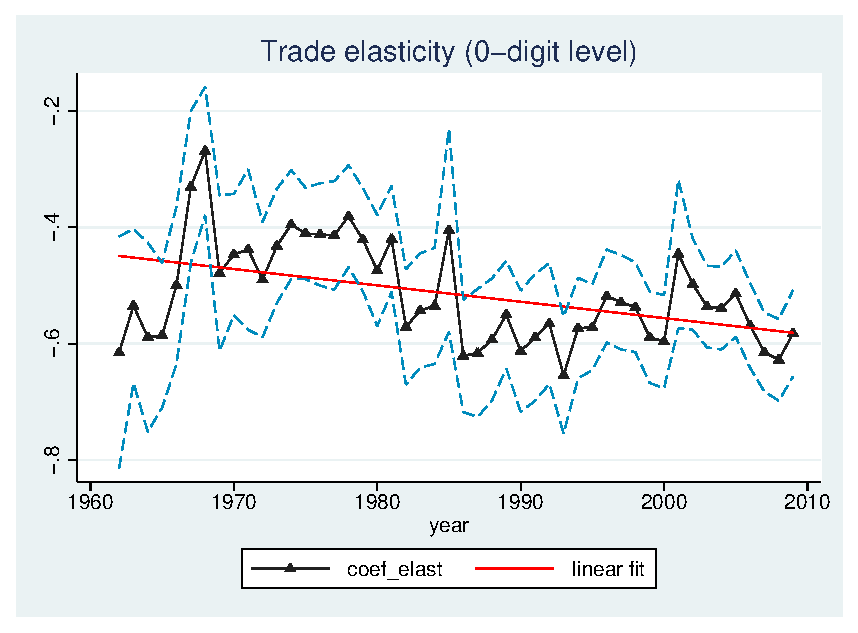
\includegraphics[trim = 0mm 0mm 0mm 9.5mm,clip,height=2.6in]{elast_real_0digit.eps}}
%\end{center}
%\caption{Estimated $(1-\widetilde{\sigma})$ \if 0 {, stepwise construction of the relative price} \fi \label{fig:elastreal0}}
%\end{figure}
%\end{frame}
%\fi
%%Figure \ref{fig:elastreal0} presents the results on the evolution of $(1-\widetilde{\sigma})$ obtained when (\ref{eqn:15}) is estimated on annual crossections of the COMTRADE dataset. The absolute value of trade elasticity has increased by 33\% from 1962 to 2009. This corresponds to an annual increase of .6\% per year.\footnote{The coefficient of the geometric fit is significant at 1\% level.} 
%\begin{frame}[plain]\frametitle{Results}
%\begin{figure}[h!]
%\begin{center}
%\setlength{\fboxrule}{1pt} %makes border lines thick
%\setlength{\fboxsep}{.1in} %increases distance to border
%%\fbox{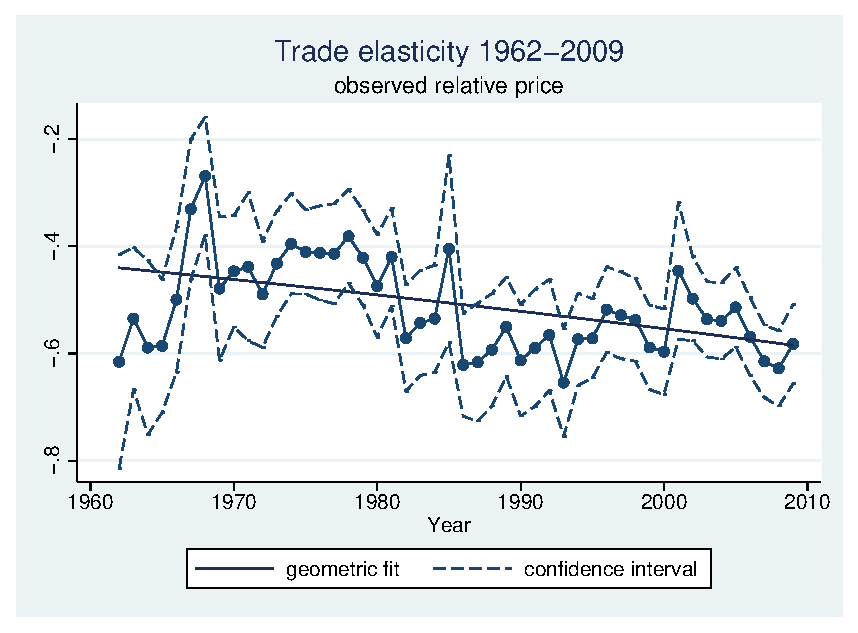
\includegraphics[0 trim = 0mm 0mm 0mm 9.5mm,clip,height=2.6in]{elast_bench.eps}}
%\fbox{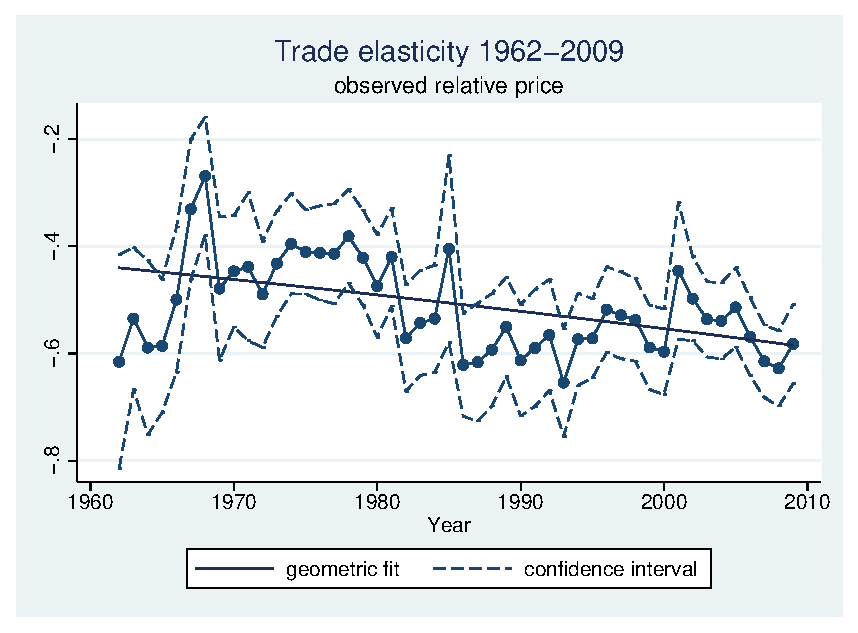
\includegraphics[height=2.5in]{elast_bench.eps}}
%\end{center}
%%\caption{Estimated $(1-\widetilde{\sigma})$ \label{fig:elastreal0}}
%\end{figure}
%\begin{itemize}
%\item 33\% increase in parameter 1962-2009
%\item corresponds to annual increase of .6\% per year 
%\end{itemize}
%\end{frame}

\subsection{Endogeneity}
%\begin{frame}[plain]\frametitle{Changing the dataset: BACI}
%\begin{figure}[h!]
%\begin{center}
%\setlength{\fboxrule}{1pt} %makes border lines thick
%\setlength{\fboxsep}{.1in} %increases distance to border
%\fbox{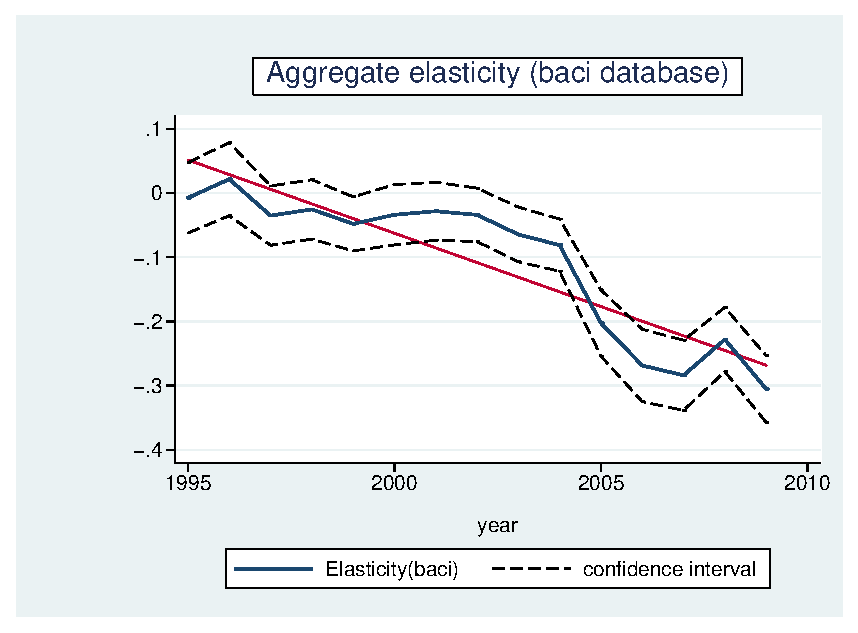
\includegraphics[height=2.5in]{elast_baci_1995_2009.eps}}
%\end{center}
%\caption{Estimated $(1-\widetilde{\sigma})$, BACI database \label{fig:baci}}
%\end{figure}
%\end{frame}
%%why baci? HS-1992 6-digit disaggregation level for 1995-2009; improved quality of relative prices of product bundles: reduced number of missing unit values (1-3\% total trade); stable share of ztf

\begin{frame}[plain]\frametitle{Instrumenting: motivation}
\vspace{0.3cm}
\begin{itemize}
	\item Unobserved demand shocks will result in increase in prices and quantities
	\begin{itemize}
		\item attenuation bias
		\item matters not only for level, but also for evolution (Feenstra(1994))
%estimated coefficient suffers from attenuation bias due to not controlling for potentially positive and finite supply elasticities
	\end{itemize}
	\item Objective: capture exporter-specific shocks to the price of the composite good which are not demand-driven
%such as exogenous shocks to the price of inputs
	\begin{itemize}
		\item GDP price level (Penn World Tables 9.0: 180 countries, 1950-2014)
		\item investment price level 
		\item price evolution in other markets
	\end{itemize}
	\item We instrument the evolution of cif unit prices by the evolution of GDP prices, investment prices and prices in other markets
	\begin{itemize}
		\item with varying number of lags
		\item we cannot produce the usual statistic tests
		\item there is a lot of noise...
		\item Still, in the second stage, between 75 and 81\% increase
	\end{itemize}
\end{itemize}
\end{frame}

\begin{frame}[plain]\frametitle{Instrumented regressions}
	\begin{figure}[h!]
		\begin{center}
			\setlength{\fboxrule}{1pt} %makes border lines thick
			\setlength{\fboxsep}{.1in} %increases distance to border
			\fbox{\includegraphics[height=2.5in]{"1ere regression 3e partie_common_axis_all_instr".pdf}}
		\end{center}
	\end{figure}
\end{frame}

%
%\begin{frame}[plain]\frametitle{Instrumenting: procedure}
%\vspace{0.3cm}
%\begin{itemize}
%\item compute relative prices for exporter-specific composite goods 
%%in each destination 
%\item compute evolution of GDP price levels of trading partners, weighted by market shares (common currency)
%%this amounts to computing the evolution of the relevant real exchange rate for each specific bilateral trade relation.
%\item compute hypothetical relative price in $t$ for each exporter as:
%\begin{itemize}
%\item product of its relative price in $(t-s)$
%\item evolution of its GDP price level between $t$ and $(t-s)$ relatively to all other partners
%\end{itemize}
%\item predict relative price of each exporter in $t$: regress observed relative price on hypothetical relative price.
%\item Idea: get an instrumented relative price which depends on past relative price and relative evolution of GDP price level.
%\item Estimate market share equation using instrumented relative prices
%%s is number of lags
%\end{itemize}
%\end{frame}
%
%\begin{frame}[plain]\frametitle{Instrumenting: one lag}
%\begin{figure}[h!]
%\begin{center}
%\setlength{\fboxrule}{1pt} %makes border lines thick
%\setlength{\fboxsep}{.1in} %increases distance to border
%\fbox{\includegraphics[height=2.5in]{elast_instr_1lag_v7.eps}}
%\end{center}
%%\caption{Estimated $(1-\widetilde{\sigma})$, instrumented relative price of composite good, 1 lag \label{fig:instr1}}
%\end{figure}
%\begin{itemize}
%\item reassuring: level of parameter increases by 9\%
%\item results on evolution hold: 13\% increase
%\end{itemize}
%\end{frame}
%%It could be argued that allowing for just one lag inadequately captures the temporal relationship between shocks to inputs' prices and their pass-through to the price of exported output. Indeed, if prices are relatively persistent, the instrumenting procedure would amount to little more than replacing observed prices in $t$ with lagged observed prices in $(t-1)$. We therefore also estimate (\ref{eqn:15}) using as instrument the evolution of each exporter's GDP price level relatively to all other trading partners in the destination between $(t-s)$ and $t$ where $s=1,...,10$.
%
%\begin{frame}[plain]\frametitle{Increasing the number of lags}
%\begin{figure}[h!]
%\begin{center}
%\setlength{\fboxrule}{1pt} %makes border lines thick
%\setlength{\fboxsep}{.1in} %increases distance to border
%\fbox{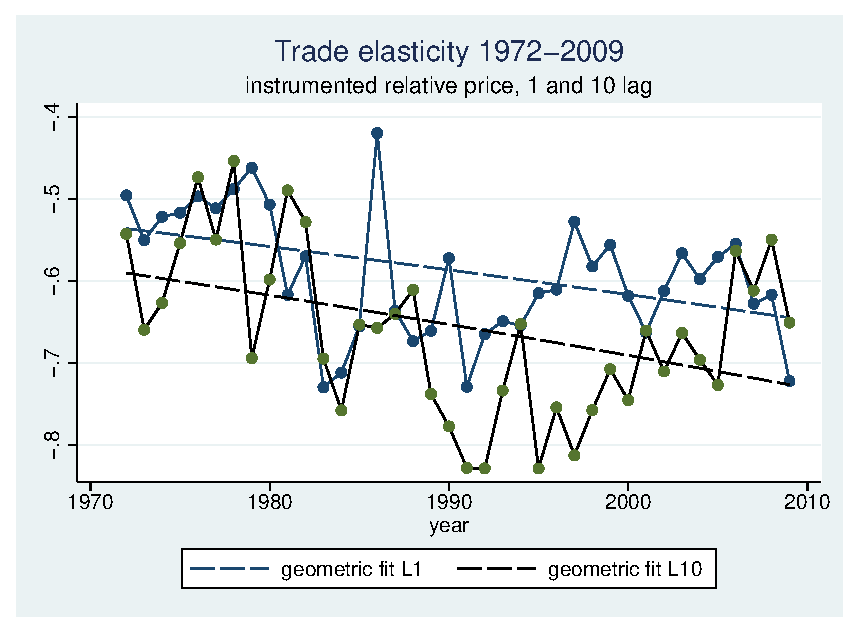
\includegraphics[height=2.5in]{elast_l1_l10.eps}}
%\end{center}
%%\caption{Estimated $(1-\widetilde{\sigma})$, instrumented relative price of composite good \label{fig:instr3}}
%\end{figure}
%\begin{itemize}
%\item level increases with number of lags: 22\% for 10 lags
%\item results on evolution hold: 23\% increase in 1972-2009 
%%(20\% for 1 lag)
%\end{itemize}
%\end{frame}
%%say: level becomes more stable as we increase nb of lags, and level increases; slope preserved
%
%\if 0
%\begin{frame}[plain]\frametitle{Increasing the number of lags}
%\begin{figure}[h!]
%\begin{center}
%\setlength{\fboxrule}{1pt} %makes border lines thick
%\setlength{\fboxsep}{.1in} %increases distance to border
%\fbox{\includegraphics[height=2.5in]{elast_instr_3_5lag_v7.eps}}
%\end{center}
%%\caption{Estimated $(1-\widetilde{\sigma})$, instrumented relative price of composite good \label{fig:instr2}}
%\end{figure}
%\begin{itemize}
%\item level increases with number of lags: 20\% for 5 lags
%\item results on evolution hold: 18\% increase in 1967-2009
%\end{itemize}
%\end{frame}
%\fi

\section{Conclusion}
\begin{frame}\frametitle{Is there a distance puzzle left?}
\begin{itemize}
\item What do we have?
	\begin{itemize}
	\item Empirical evidence on 22 to 81\% increase in substitutability parameter
	\item This is aggregate trade elasticity in Armington framework
	\item Combined with a 4.5 to 31\% increase in distance elasticity
	\item Provides a direct explanation of the distance puzzle
	\end{itemize}
\item What is going on?
	\begin{itemize}
	\item Perceived increasing similarity in the country-specific bundles
	\item Because of the declining importance of location-specific primary products?
	\item Because of the geographical dispersion of development?
	\end{itemize}
\end{itemize}
\end{frame}


\begin{frame}[plain]\frametitle{About FTA}
	\begin{figure}[h!]
		\begin{center}
			\setlength{\fboxrule}{1pt} %makes border lines thick
			\setlength{\fboxsep}{.1in} %increases distance to border
			\fbox{\includegraphics[height=2.5in]{"fta_proximity".pdf}}
		\end{center}
	\end{figure}
\end{frame}

\end{document}